
\documentclass[]{article}

\usepackage{xspace}
\usepackage{hyperref}
\usepackage{graphicx}
\usepackage{subcaption}
\usepackage[a4paper, total={6in, 9in}]{geometry}

% Define a few constants used in the report that we can change here if needed
\newcommand{\winningaccuracy}{86\%\xspace}
\newcommand{\winningtpaccuracy}{90\%\xspace}
\newcommand{\winningfnrate}{10\%\xspace}
\newcommand{\winningmodelshort}{RF\xspace}
\newcommand{\winningmodellong}{Random Forest\xspace}
\newcommand{\winningtnrate}{73\%\xspace}

% Title Page
\title{Understanding, predicting and preventing Churn}
\author{William RJ Cooper}


\begin{document}
\maketitle

\section{Executive Summary}

In this report we outline a model that can predict whether a customer will leave a business or not (churn) with around \winningaccuracy accuracy, using a few pieces of information readily available to most banks. Preventing churn is vital in most businesses, and predicting it is the first step. This report outlines a model that:

\begin{itemize}
	\item can predict customer churn can be predicted with \winningaccuracy accuracy
	\item can output a percentage indicating how likely the customer is to leave or stay
	\item has a low false negative rate (\winningfnrate) meaning it is unlikely for the model to predict that a churning customer will stay
\end{itemize}

This model for predicting customer churn and assigning a confidence value can be used to offer pre-made tiered packages to customers, with scaling value for money meaning that customers most likely to churn can be offered the most lucrative discounts or products to keep them from churning.

\section{Introduction}

Churn, customer attrition, customer retention, all refer to the loss of customers from a business. Henceforth referred to as simply churn, minimising the loss of customers from any business is beneficial to any business for several reasons:

\begin{itemize}
	\item It can cost \href{https://www.forbes.com/sites/jiawertz/2018/09/12/dont-spend-5-times-more-attracting-new-customers-nurture-the-existing-ones/#47efa3d45a8e}{5 times more} to acquire and sign a new customer than retain an existing one
	\item According to a report by Harvard Business School, ‘increasing customer retention rates by 5\% \href{https://hbswk.hbs.edu/archive/the-economics-of-e-loyalty}{increases profits by 25\% to 95\%}’
	\item 80\% of your future profits will come from just 20\% of your existing customers (Leading on the Edge of Chaos: The 10 Critical Elements for Success in Volatile Times by Emmett C. Murphy, Mark A. Murphy, 978-0735203129)
\end{itemize}

Any scheme that seeks to understand, predict and prevent customer churn may be able to increase profits, reduce costs and increase customer satisfaction. 

Businesses often keep large amounts of data about their customers, and whether or not a customer has churned would also be easy to calculate. It is for this reason that this problem is perfect for data-driven solution as if there is a link between customer data and churn, these methods can find it.

In this research we choose two datasets containing various information about customers including whether or not they have churned. Even though these datasets are from bank customers and I am not in banking myself, there is no reason why the approach we use here could not be used for other datasets from businesses in other areas. This is why I chose this project, because customer churn affects almost every business. 

The ultimate aim of this research is to create a model that, given certain customer attributes will predict whether a customer will churn or not. Our final model also has some benefits over other models that it also outputs a confidence value based on how likely it is to be correct, and can be interpreted as a value showing how likely it is that a customer will churn or not. This has the added benefit that this confidence value could be used to implement a tiered system to offer increasingly valuable products or discounts to customers who are likely to churn. The more likely a customer is to churn, the bigger the discount they can be offered to entice them to stay.

\section{Methods}

\subsection{Datasets}

In this section we present an overview of the steps taken from cleaning all the way to applying models to the data. For more detail, please see the source code \href{https://github.com/ray33ee/Understanding-predicting-and-preventing-churn/blob/main/Customer%20Churn%20Analysis.ipynb}{here}.

In our journey to predict customer churn we will focus on two datasets:

\begin{itemize}
	\item \href{https://www.kaggle.com/datasets/gauravtopre/bank-customer-churn-dataset}{Dataset A}
	\item \href{https://www.kaggle.com/datasets/willianoliveiragibin/bank-churn-prediction}{Dataset B}
\end{itemize}

These datasets both contain attributes and information on their customers, and whether they have churned from the bank. These datasets have 11 attributes in common, namely:

\begin{itemize}
	\item \textbf{Age} - Stored as a single number
	\item \textbf{Credit score} – A number between 0 and 999
	\item \textbf{Country} – Either France, Germany or Spain. Country is stored differently in both sets, one stores it as a string, and one stores as as three separate columns with a ‘1’ indicating that country. We will use the latter strategy, so the former dataset will have to be modified to reflect this. This can be implemented trivially in Python
	\item \textbf{Gender} – Stored as ‘Male’ or ‘Female’ in one source, and as two columns in the second. Once again the approach of having two columns will be used.
	\item \textbf{Tenure} – The number of years the customer has been with the bank
	\item \textbf{Account Balance} – Customer bank balance
	\item \textbf{Number of Products} – Number of financial products the customer has purchased from the bank
	\item \textbf{Credit Card} – 0 or 1 depending on if they have a credit card or not
	\item \textbf{Estimated salary} – Number indicating salary
	\item \textbf{Active Member} – 1 if the customer is active and using their account, 0 if not
	\item \textbf{Customer Churn} – 1 indicating that the customer has left the bank, 0 indicating they are still a customer
\end{itemize}

There are certain attributes that are deemed irrelevant (such as the names of the customers), redundant (attributes that are composites of other attributes, such as the Age/Tenure product) and also attributes that are not common to both datasets. These attributes we omit, sticking to the 11 mentioned above. This forms the first step for merging the datasets, only keep attributes that are common to both and drop all others.

\subsection{Cleaning}

In this subsection we outline the methods for cleaning and merging then removing outliers and normalising the combined datasets.

\subsubsection{Loading}

On downloading and reading the CSV files into dataframes, pandas gives a warning that columns have mixed types for dataset B. This will be addressed in the next section, for now we drop columns that are not present in both datasets to leave us with the columns we will use.

\subsubsection{Invalid Numbers}

On further inspection we see that the columns for credit score, age, tenure and number of products are all floating values. This is mostly due to formatting (These values are floating in the csv files) but there are also some invalid numbers in the age and the estimated salary columns. To solve this, we create some helper functions that convert a value into a floating number, and integer or a binary value. If the conversion fails, we replace the number with null. After we apply the appropriate conversion for each column, we then drop all entries containing null values effectively removing entries with invalid formatting. We then convert the columns to the correct types, integers for credit score, age, tenure and number of products. We also take this time to check for NaN values, but none exist so no further action is needed.

\subsubsection{One-hot encoding}

The Country and gender columns in dataset A store these attributes as string values. Since we are using statistical techniques that will not work with this format, we use one-hot encoding to convert the categorical data into numerical.

\subsubsection{Renaming columns}

The columns are labelled differently in both datasets, so we create a mapping of old columns names to new column names, and apply this to both datasets so columns representing the same data will have the same name.

\subsubsection{Types}

At this point we check the dtype of all the columns, which are floating for AccountBalance and EstimatedSalary, and integer for the rest as expected.

\subsubsection{Merging}

At this point the datasets have been cleaned, null values removed, and column names synced up so the datasets are concatenated into a single dataframe.

\subsubsection{Shuffle}

To remove any bias that may exist in entering the values, and that certainly exists by concatenating the two different datasets, we shuffle the dataset.

\subsubsection{Outliers}

Using the IQR test for detecting outliers on the following attributes:

\begin{itemize}
	\item Age
	\item Tenure
	\item Credit Score
	\item Account balance
	\item Estimated Salary
	\item Number of products
	\item Has credit card?
	\item Is active member
\end{itemize}

And this identifies 6690 outliers namely from the ‘Credit Score’, ‘Age’ and ‘Number of products’ attributes, which we remove from the dataset

\subsubsection{Normalising}

Finally, since most of the techniques require the data to be normalised, we do this for all attributes (Except customer churn which must remain categorical) by subtracting the mean and dividing my the standard deviation for all columns.

\subsection{Visualising}

Now the data is cleaned and normalised we can apply 2 component and 3 component PCA analysis on the data (we do not use the ‘Churn’ columns in PCA) and plot the data on 2D and 3D scatter plots, respectively, and colour by churn. This gives us a way to visualise the multi-dimensional data, and hopefully allow us to see a difference between churned and non-churned data. Visualising PCA will give us a clue as to how easy the data will be to classify, as if churned and non-churned data has little overlap, then this is a strong indicator that the data will be easy to classify.

\subsection{Models}

Now that the data is ready to be analysed, we split the data into training and validation sets and apply a range of models to the data. Our goal in this is of course to predict churn, which comes in two categories, churned and not churned. Because of this, the types of models we use are classifiers and regression models. In this analysis we try 9 different models and compare their effectiveness, namely:

\begin{itemize}
	\item \href{https://github.com/microsoft/LightGBM}{LightGBM} (LGBM) - A fast gradient boosting framework based on decision trees
	\item \href{https://scikit-learn.org/stable/modules/generated/sklearn.linear_model.LogisticRegression.html}{Logistic Regression} (LR)
	\item \href{https://scikit-learn.org/stable/modules/generated/sklearn.ensemble.RandomForestClassifier.html}{Random Forest classifier} (RF)
	\item \href{https://scikit-learn.org/stable/modules/generated/sklearn.ensemble.GradientBoostingClassifier.html}{Gradient Boosting classifier} (GBC)
	\item \href{https://scikit-learn.org/stable/modules/generated/sklearn.neural_network.MLPClassifier.html}{MLP classifier} (MLP)
	\item \href{https://scikit-learn.org/stable/modules/generated/sklearn.ensemble.AdaBoostClassifier.html}{Ada Boost classifier} (ADA)
	\item \href{https://scikit-learn.org/stable/modules/generated/sklearn.neighbors.KNeighborsClassifier.html}{K-nearest neighbours} (KNN)
	\item \href{https://scikit-learn.org/stable/modules/generated/sklearn.discriminant_analysis.LinearDiscriminantAnalysis.html}{Linear Discriminant Analysis} (LDA)
	\item \href{https://keras.io/api/models/sequential/#sequential-class}{Convolutional Neural Network} (CNN) - Keras implementation of a sequential CNN model
\end{itemize}

\newpage

\section{Results}

Our first graph simply shows the ratio of churned to not churned customers in the dataset:

\begin{figure}[h!]
	\centering
	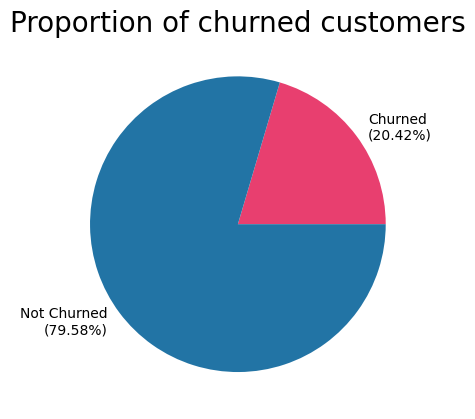
\includegraphics[scale=0.5]{churn_proportion}
	\caption{Pie chart showing the proportion of the dataset that is churned (20.42\%) against the proportion that is not churned (79.58\%) (\href{https://github.com/ray33ee/Understanding-predicting-and-preventing-churn/blob/main/tex/churn_proportion.png?raw=true}{larger image})}
\end{figure}

As we can see the dataset is heavily biased towards customers who have not churned. This is not surprising as, at least for successful companies, churn should be low. This bias is very important to keep in mind however, since optimising models to predict churn could result in finding local solutions which simply guess ‘not churn’ and do not predict at all. Because of the bias in the dataset, a model which trivially predicts ‘not churned’ would have an accuracy of around 80\%. Later on we discuss how we can look out for models that do this, and we even see an example of a poor neural network which takes this approach but looks to have a high accuracy.

For the next few charts we compare the churned vs non-churned samples over various attributes including age, activity, number of products purchased, account balance, estimated salary, credit score and tenure. First we see the age attribute, which has the most obvious differences for churn and non churned customers:

\begin{figure}[h!]
	\centering
	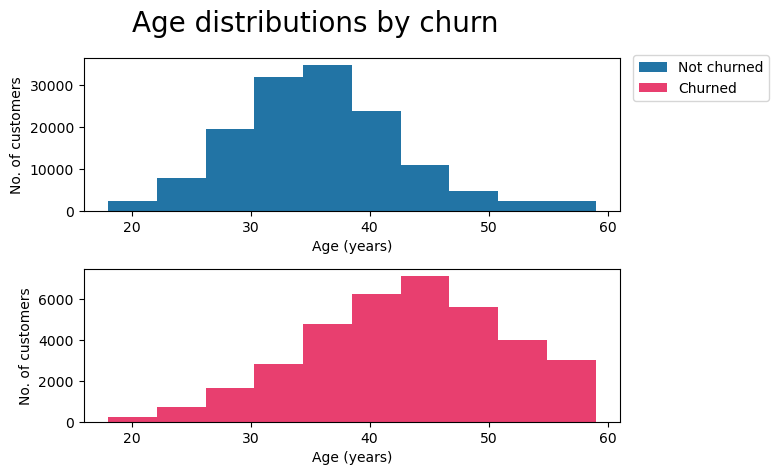
\includegraphics[scale=0.4]{age_by_churn}
	\caption{Histogram showing the distribution of age for non churned customers that has a positive skew, and a second histogram showing the distribution for churned customers which skews negatively. (\href{https://github.com/ray33ee/Understanding-predicting-and-preventing-churn/blob/main/tex/age_by_churn.png?raw=true}{larger image})}
\end{figure}

As we will see not all plots show any correlation, but in this case there seems to be a strong link between age and churn. The not churned histogram skews left, showing a younger age, whereas the churned histogram skews right, possibly meaning that churned customers are older than not churned. Next we have customer activity:

\clearpage

\begin{figure}[h!]
	\centering
	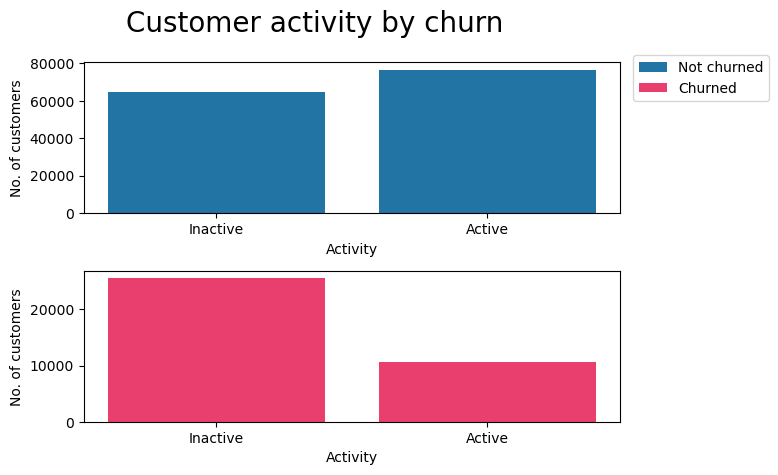
\includegraphics[scale=0.5]{activity_by_churn}
	\caption{Histogram showing the distribution of age for non churned customers that has a positive skew, and a second histogram showing the distribution for churned customers which skews negatively. (\href{https://github.com/ray33ee/Understanding-predicting-and-preventing-churn/blob/main/tex/activity_by_churn.png?raw=true}{larger image})}
\end{figure}

Here we see that vastly more users are inactive in the churned group which could suggest that inactivity leads to churn. However, it is important to note here that we cannot say which way the correlation flows, and indeed in this case it is more likely that the explanation is that customers who leave become inactive. If the causation does flow this way, customer activity may not be an accurate way to predict churn, as churn may come after inactivity. Up next is a plot of the number of products purchased by customers:

\begin{figure}[h!]
	\centering
	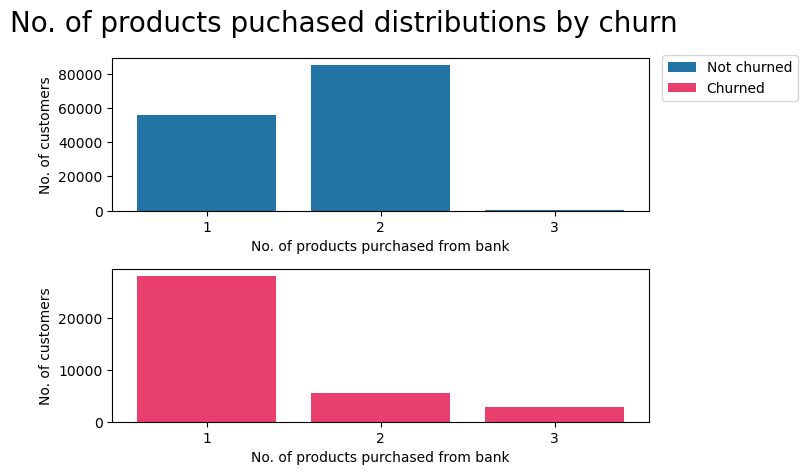
\includegraphics[scale=0.5]{products_by_churn}
	\caption{Histogram showing the distribution of age for non churned customers that has a positive skew, and a second histogram showing the distribution for churned customers which skews negatively. (\href{https://github.com/ray33ee/Understanding-predicting-and-preventing-churn/blob/main/tex/products_by_churn.png?raw=true}{larger image})}
\end{figure}

Here again we see big differences between churn and not churned customers, namely that it is much more common for not-churned customers to have purchased more than one product. Purchasing more than one product could be a big indicator that a customer won’t churn. Finally we have plots for the other features, however these plots do not seem to show many differences between churn and not-churn so warrant no further discussion:
\clearpage

\begin{figure*}[t!]
	\centering
	\begin{subfigure}[t]{0.55\textwidth}
		\centering
		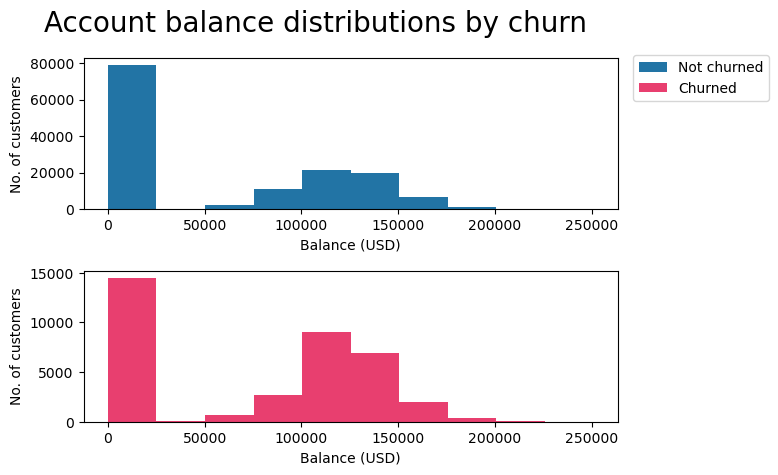
\includegraphics[height=2in]{account_balance_by_churn}
		\caption{Account balances for churn and non-churned customers  (\href{https://github.com/ray33ee/Understanding-predicting-and-preventing-churn/blob/main/tex/account_balance_by_churn.png?raw=true}{larger image})}
	\end{subfigure}%
	~ 
	\begin{subfigure}[t]{0.5\textwidth}
		\centering
		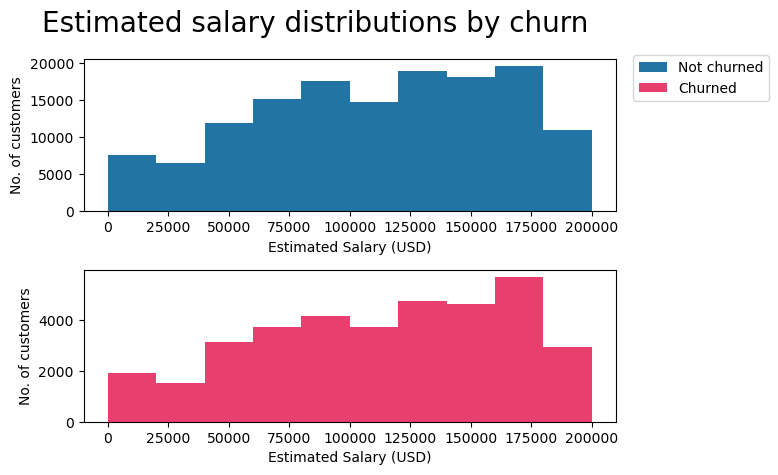
\includegraphics[height=2in]{estimated_salary_by_churn}
		\caption{Estimated salaries for churn and non-churned customers (\href{https://github.com/ray33ee/Understanding-predicting-and-preventing-churn/blob/main/tex/estimated_salary_by_churn.png?raw=true}{larger image})}
	\end{subfigure}
	
	\begin{subfigure}[t]{0.55\textwidth}
		\centering
		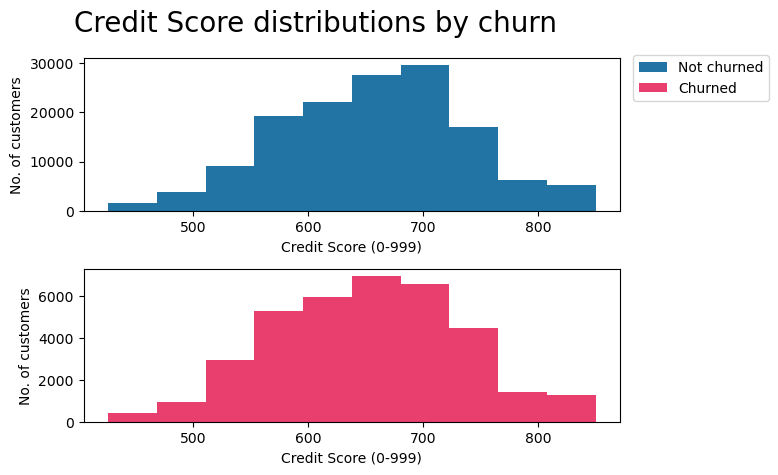
\includegraphics[height=2in]{credit_score_by_churn}
		\caption{Credit scores for churn and non-churned customers (\href{https://github.com/ray33ee/Understanding-predicting-and-preventing-churn/blob/main/tex/credit_score_by_churn.png?raw=true}{larger image})}
	\end{subfigure}%
	~
	\begin{subfigure}[t]{0.5\textwidth}
		\centering
		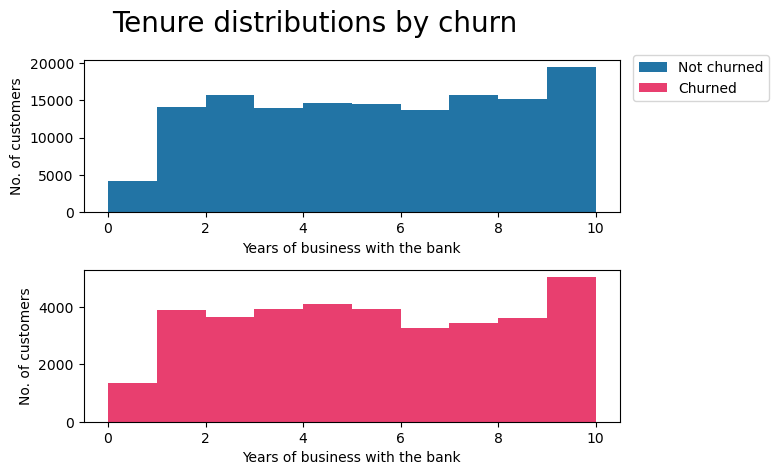
\includegraphics[height=2in]{tenure_by_churn}
		\caption{Tenures for churn and non-churned customers (\href{https://github.com/ray33ee/Understanding-predicting-and-preventing-churn/blob/main/tex/tenure_by_churn.png?raw=true}{larger image})}
	\end{subfigure}
	\caption{Frequency distributions by churn for account balance (a), estimated salary (b), credit scores (c) and tenure (d) showing no real difference between churn and non-churned customers}
\end{figure*}

The final section of our descriptive statistics analysis summarises the plots we have seen so far with a correlation matrix:

\begin{figure}[h!]
	\centering
	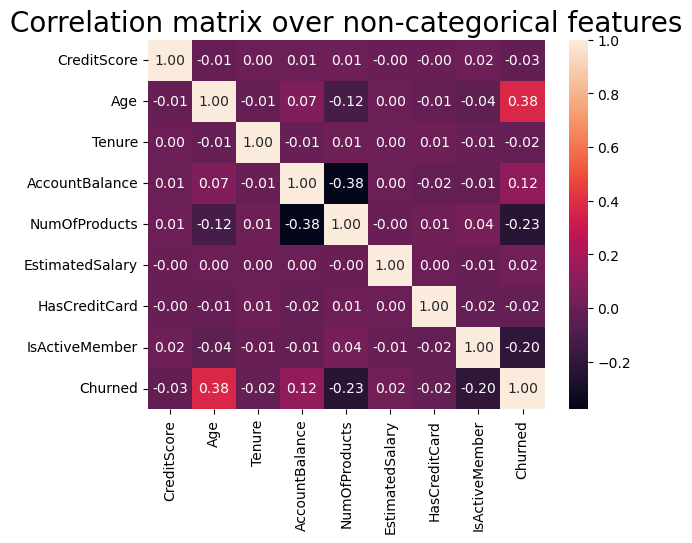
\includegraphics[scale=0.46]{correlation}
	\caption{Correlation matrix for all attributes showing a correlation between churn and age, account balance, number of products and activity (\href{https://github.com/ray33ee/Understanding-predicting-and-preventing-churn/blob/main/tex/correlation.png?raw=true}{larger image})}
\end{figure}

This correlation matrix confirms what we have seen so far, namely a correlation with churn against Age, number of products and activity, it also shows a correlation with tenure too.

These results are extremely promising, as they show that the data is correlated and connected and that optimisation may be used to predict churn.

Before we start optimising, our last step is to use PCA to reduce the dimensionality of the dataset to 2 or 3 dimensions, then plot these points on 2D and 3D scatter graphs, colouring points based on churn. Here are the results:

\begin{figure*}[h!]
	\centering
	\begin{subfigure}[t]{0.55\textwidth}
		\centering
		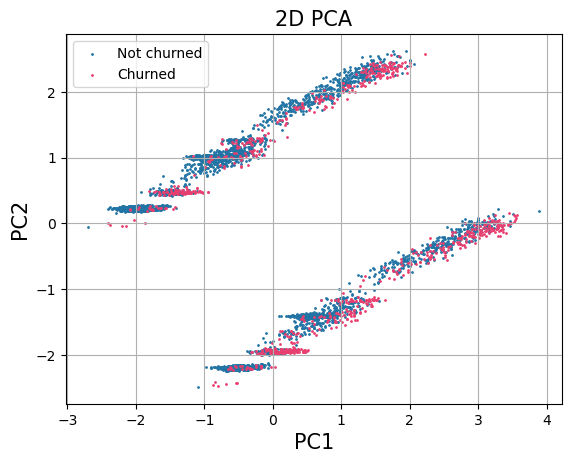
\includegraphics[height=3in]{2d}
		\caption{2D PCA visualisation with points coloured by churn (\href{https://github.com/ray33ee/Understanding-predicting-and-preventing-churn/blob/main/tex/2d.png?raw=true}{larger image})}
	\end{subfigure}
	\begin{subfigure}[t]{0.55\textwidth}
		\centering
		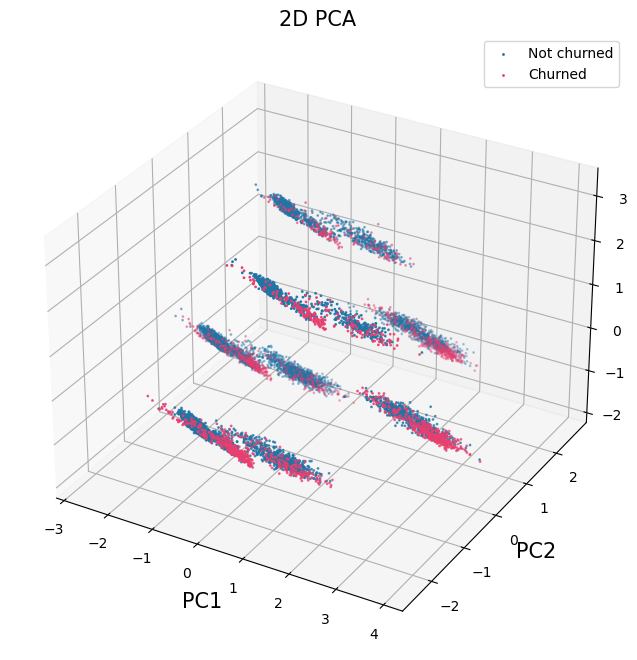
\includegraphics[height=3in]{3d}
		\caption{3D PCA visualisation with points coloured by churn (\href{https://github.com/ray33ee/Understanding-predicting-and-preventing-churn/blob/main/tex/3d.png?raw=true}{larger image})}
	\end{subfigure}
	\caption{2D (a) and 3D (b) PCA visualisations showing no visible pattern between churn and non churned data points}
\end{figure*}

Since we removed churn from the PCA analysis, any differences in the churned vs not churned points would entirely be from the features and not churn itself. However, as we see from the plots, there are no discernable differences and there is a great overlap in the data. 

As PCA has not given any extra insight into our dataset, we move on to applying our 9 models on the dataset to see if there is any way to extract meaning from the data. We summarise our results with confusion tables from predictions for all 9 models:

\begin{figure}[h!]
	\centering
	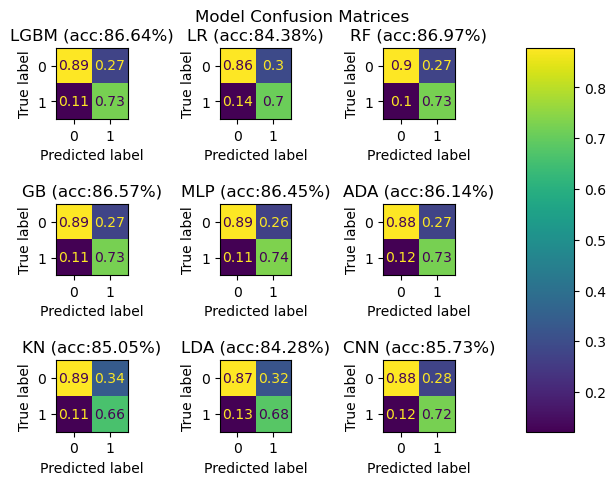
\includegraphics[scale=0.6]{9cm}
	\caption{Confusion matrices (by percentage prediction) for all 9 models used, displaying accuracy and model type too (\href{https://github.com/ray33ee/Understanding-predicting-and-preventing-churn/blob/main/tex/9cm.png?raw=true}{larger image})}
\end{figure}

There is a lot going on in this one plot, so lets start with the \winningmodellong model confusion matrix:

\begin{figure}[h!]
	\centering
	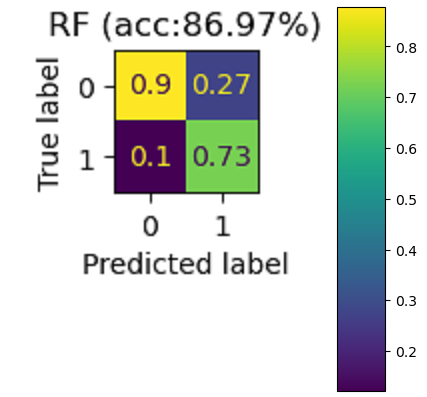
\includegraphics[scale=1]{rf_cm}
	\caption{Confusion matrices  for \winningmodellong (\winningmodelshort) which has the highest accuracy (\winningaccuracy) the best false negative rate (\winningfnrate) and the best true positive accuracy (\winningtpaccuracy) (\href{https://github.com/ray33ee/Understanding-predicting-and-preventing-churn/blob/main/tex/rf_cm.png?raw=true}{larger image})}
\end{figure}

First we note that the confusion matrix does not show integer values in the table, but decimals. This is because we show the percentage based on the predicted label. So in the \winningmodelshort example, when the model predicted a ‘0’ is was correct \winningtpaccuracy of the time, and when it predicted a ‘1’ it was correct \winningtnrate of the time. Presenting the matrix in this was is important as the dataset is very biased towards not churn, so showing the results as percentages removes this bias. It also shows us the percentage of time the model is a true positive. This is important as for models that guess randomly this value will be about 20\%, and for models that predict 0 this will be 0\%. Getting a high percentage (\winningtnrate in this case) is enough to convince us that this is not guesswork. We also see the overall accuracy of this model, \winningaccuracy. 

While some models are slightly better than others, they are all around 86\% accurate, even the models that are fundamentally different show no higher than 87\%. This, I suspect is the upper bound of the dataset itself, to have multiple models so closely agree on an accuracy must mean that they cannot extract any more meaning from the data.

For comparison, we now show two confusion matrices of trivial models, the first guesses uniformly randomly for churned/not churned, and the second always guesses not churned:

\begin{figure*}[h!]
	\centering
	\begin{subfigure}[t]{0.55\textwidth}
		\centering
		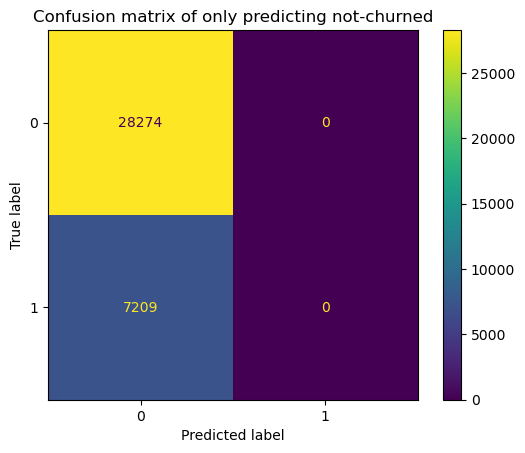
\includegraphics[height=2.7in]{trivial_0}
		\caption{Confusion matrix of a model which guesses 'not churned' every time, showing a true positive rate of 0\% but an overall accuracy of around 80\%  (\href{https://github.com/ray33ee/Understanding-predicting-and-preventing-churn/blob/main/tex/trivial_0.png?raw=true}{larger image})}
	\end{subfigure}%
	~
	\begin{subfigure}[t]{0.55\textwidth}
		\centering
		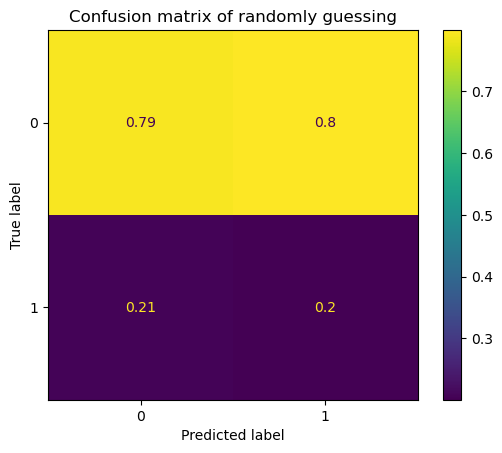
\includegraphics[height=2.7in]{trivial_guesser}
		\caption{Confusion matrix of a model which guesses uniformly randomly, showing a true positive rate of 20\% (\href{https://github.com/ray33ee/Understanding-predicting-and-preventing-churn/blob/main/tex/trivial_guesser.png?raw=true}{larger image})}
	\end{subfigure}
	\caption{Confusion matrices of poor trivial models that may have high overall accuracies (80\% in both cases) but very poor true positive rates (under 20\%)}
\end{figure*}

\section{Conclusion}

To get an idea of which models might be better than others we train classifiers, regression models, a neural network model and random forest classifiers on a training set then evaluate their effectiveness based on three main factors:

\begin{enumerate}
	\item Overall accuracy on the validation set
	\item True positive accuracy
	\item Does the model output a yes/no or a more helpful confidence value?
	\item False negative rate
\end{enumerate}

Checking the true positive accuracy is very important because the dataset is about 80\% composed of customers who have not churned, and 20\% who have. This means that a model that always guesses not churned would be 80\% accurate. This model is of course highly undesirable, and it would have a true positive accuracy of 0\%. Getting this true positive accuracy as high as possible is what makes an accurate model and proves to be difficult. The third factor is important because it gives more information on the customer (how likely they are to churn or not churn) which can be used to prescribe an outcome more tailored to that customer (Heavy discounts, personalised products, reaching out personally via customer service, etc.). Finally the false negative rate is important because it shows us how many customers the model will predict will stay when in fact they churn. Since this is the worst case outcome, minimising this is important.

From our results we see that the best for accuracy is the \winningmodelshort model, and the best true positive is the \winningmodelshort model. Finally since the CNN is the only model that outputs a confidence value, we see that \winningmodelshort and CNN models are our best bet for the three questions. To give the best of both, I propose a hybrid model which combines the best of both by using the result of \winningmodelshort with the confidence value from CNN, if it agrees with the \winningmodelshort result, if not, no confidence value is provided.

The best model for false negatives is \winningmodelshort. This represents the cases where the model predicts a customer will not leave when they do. This is certainly a worst case scenario as it will result in customers leaving without the model predicting it. Needless to say this metric should be as low as possible, we are fortunate that the rates are low, at \winningfnrate for the \winningmodelshort model.

Finally we propose a list of next steps:

\begin{enumerate}
	\item Create a python application that applies the model we have chosen and takes customer data and outputs a value indicating a prediction on churn
	\item Implement this algorithm in the company to predict churn on all customers and also apply it anytime the data changes for a customer (increased age, another product purchased, etc.)
	\item Use the prediction to decide the best course of action for customers who are predicted to churn. If the chosen model outputs a yes/no answer, then choose and apply an action for customers predicted to churn. If the chosen model gives a confidence value, create and apply a tiered solution that maps confidence values to prescribed actions
	\item Finally keep track of churn percentages before and after the model is implemented to evaluate the models’ success
\end{enumerate}

\section{Evaluation}

Overall the accuracy of the models are reasonably high, and this shows that it is possible to predict churn from the data. However it would be ideal to get an accuracy above \winningaccuracy, and here are some steps we could take to achieve this:

\begin{enumerate}
	\item Include more customer features, such as 
	\begin{itemize}
		\item number of complaints
		\item customer service rating
		\item support rating
		\item time since last activity on account
		\item how much money borrowed from bank
		\item number of promotional offers received
	\end{itemize}
	\item Include more diverse customers, such as customers from other countries, religions, etc.
\end{enumerate}

\end{document}          
